\documentclass[10pt,a4paper,draft]{article}
\usepackage[utf8x]{inputenc}
\usepackage{ucs}
\usepackage[english]{babel}
\usepackage{multirow}
\usepackage{rotating}
\author{Lukáš Petrovický}
\title{RAS2012: Competition Entry}
\begin{document}

\maketitle

\begin{abstract}
This article describes an entry to the 2012 RAS Problem Solving Competition, concerning dispatching on multi-track territories. The entry is based on the Drools Planner, a Java-based solver. On a reasonably recent computer, the resulting algorithm is able to produce feasible results within a minute and has been fine-tuned to provide best results in under 3 minutes. Source code to the entry is open source and well documented.
\end{abstract}

\section{Introduction}

\section{Describing the solution}

\section{Implementation}

\section{Achieved results}

Running the algorithm described above 20 times over each data set, we have compiled a set of results, see Table \ref{table:result}. All these were reached within 3 minutes in a single-threaded run, using Intel i7 Q820 processor running Fedora 17 and 2 GB of heap space inside Java 7 runtime environment.

\begin{table}
\footnotesize
\caption{Submission performance per data set.}
\centering
\begin{tabular}{c||c|c|c|c|c}
\hline \hline
                 & Best                 & Q1                 & Q2                & Q3                & Worst \\ 
\hline
TOY & \$1074   & \$1074   & \$1074  & \$1074  & \$1074 \\
\hline
RDS1 & \$2056   & \$2251   & \$2561.5  & \$3385  & \$4628 \\
\hline
RDS2 & \$7895   & \$9270   & \$9851.5  & \$10600  & \$12462 \\
\hline
RDS3 & \$10257   & \$11194   & \$11816  & \$12396  & \$14135 \\
\end{tabular} 
\label{table:result} 
\end{table}

\begin{figure}
\centering
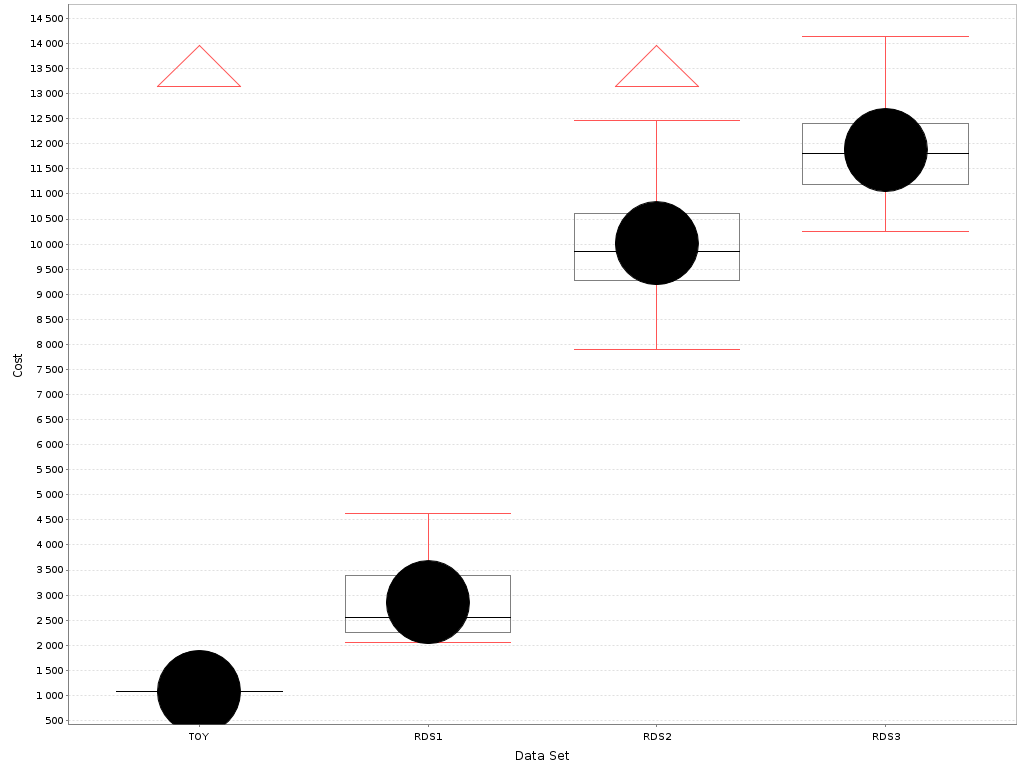
\includegraphics[width=120mm]{chart.png}
\caption{Plotting the data for the various resolved systems.}
\end{figure}

Please note that via the benchmarking functionality of Drools Planner, users may be able to fine-tune the algorithm to be focused either on providing better solutions or on faster turnaround times. Drools Planner even allows for retrieving the intermediate results of the algorithm and also modify the problem while it's being solved, which makes it the ideal tool for real-time planning.

For statistics of the resolved systems, see tables \ref{table:TOY-808.tex}, \ref{table:RDS1-996.tex}, \ref{table:RDS2-7597.tex} and \ref{table:RDS3-11023.tex} respectively. 

\section{Conclusion}

\appendix

\section{Resolved systems}

In this section, we show the best solutions reached for each data set. 

\begin{sidewaystable}
\centering
\footnotesize
\caption{Statistics for resolved system ``RAS DATA SET TOY'', costing \$808.}
\begin{tabular}{c||c|c||c|c|c|c|c||c|c|c}
  \hline \hline
  &
  Unpref. & 
  Delay &
  Node &
  When &
  SA &
  +/- &
  Pty &
  TWT &
  +/- &
  Pty \\
      \hline
      \multirow{2}{*}{A1} &
      \multirow{2}{*}{0} &
      \multirow{2}{*}{1260} &
      6 &
      4260 &
      2400 &
        -1860 &
        0 &
      \multirow{2}{*}{8700} &
        \multirow{2}{*}{2640} &
        \multirow{2}{*}{0}
      \\
      \cline{4-8}
       &
       &
       &
      12 &
      6060 &
      4800 &
        -1260 &
        0 &
      
         &
        
      \\
      \hline
      \multirow{2}{*}{B1} &
      \multirow{2}{*}{0} &
      \multirow{2}{*}{3480} &
      6 &
      6283.16 &
      -3000 &
        -9283.16 &
        115 &
      \multirow{2}{*}{4800} &
        \multirow{2}{*}{-3903.328} &
        \multirow{2}{*}{0}
      \\
      \cline{4-8}
       &
       &
       &
      0 &
      8703.328 &
      5400 &
        -3303.328 &
        0 &
      
         &
        
      \\
      \hline
      \multirow{2}{*}{C1} &
      \multirow{2}{*}{0} &
      \multirow{2}{*}{0} &
      6 &
      2400 &
      3000 &
        600 &
        0 &
      \multirow{2}{*}{7200} &
        \multirow{2}{*}{2400} &
        \multirow{2}{*}{0}
      \\
      \cline{4-8}
       &
       &
       &
      12 &
      4800 &
      6000 &
        1200 &
        0 &
      
         &
        
      \\
\end{tabular}
\label{table:TOY-808.tex} 
\end{sidewaystable}

\begin{sidewaystable}
\centering
\footnotesize
\caption{Statistics for resolved system ``RAS DATA SET 1'', costing \$996.}
\begin{tabular}{c||c|c||c|c|c|c|c||c|c|c}
  \hline \hline
  &
  Unpref. & 
  Delay &
  Node &
  SA &
  Actual &
  +/- &
  Pty &
  TWT &
  +/- &
  Pty \\
      \hline
      \multirow{2}{*}{A1} &
      \multirow{2}{*}{0} &
      \multirow{2}{*}{0} &
      37 &
      3600 &
        3172.5 &
        427.5 &
        0 &
      \multirow{2}{*}{5400} &
        \multirow{2}{*}{-319.5} &
        \multirow{2}{*}{0}
      \\
      \cline{4-8}
       &
       &
       &
      39 &
      7800 &
        5719.5 &
        2080.5 &
        0 &
      
         &
        
      \\
      \hline
      \multirow{2}{*}{A2} &
      \multirow{2}{*}{0} &
      \multirow{2}{*}{1740} &
      37 &
      7800 &
        7384.742 &
        415.258 &
        0 &
      \multirow{2}{*}{9000} &
        \multirow{2}{*}{-1542.01} &
        \multirow{2}{*}{0}
      \\
      \cline{4-8}
       &
       &
       &
      39 &
      12000 &
        10542.01 &
        1457.99 &
        0 &
      
         &
        
      \\
      \hline
      \multirow{2}{*}{B1} &
      \multirow{2}{*}{16} &
      \multirow{2}{*}{0} &
      37 &
      12600 &
        10838.335 &
        1761.665 &
        0 &
      \multirow{2}{*}{13800} &
        \multirow{2}{*}{-857.372} &
        \multirow{2}{*}{0}
      \\
      \cline{4-8}
       &
       &
       &
      0 &
      17400 &
        14657.372 &
        2742.628 &
        0 &
      
         &
        
      \\
      \hline
      \multirow{2}{*}{B2} &
      \multirow{2}{*}{0} &
      \multirow{2}{*}{0} &
      37 &
      15600 &
        14264.466 &
        1335.534 &
        0 &
      \multirow{2}{*}{16800} &
        \multirow{2}{*}{-448.224} &
        \multirow{2}{*}{0}
      \\
      \cline{4-8}
       &
       &
       &
      39 &
      19800 &
        17248.224 &
        2551.776 &
        0 &
      
         &
        
      \\
      \hline
      \multirow{2}{*}{B3} &
      \multirow{2}{*}{14} &
      \multirow{2}{*}{1680} &
      37 &
      40200 &
        40937.661 &
        -737.661 &
        0 &
      \multirow{2}{*}{42000} &
        \multicolumn{2}{c}{\multirow{2}{*}{N/A}}
      \\
      \cline{4-8}
       &
       &
       &
      39 &
      45000 &
        \multicolumn{3}{|c||}{N/A} &
      
        
      \\
      \hline
      \multirow{2}{*}{C1} &
      \multirow{2}{*}{0} &
      \multirow{2}{*}{0} &
      37 &
      19200 &
        17598 &
        1602 &
        0 &
      \multirow{2}{*}{21600} &
        \multirow{2}{*}{282} &
        \multirow{2}{*}{0}
      \\
      \cline{4-8}
       &
       &
       &
      39 &
      24600 &
        21318 &
        3282 &
        0 &
      
         &
        
      \\
      \hline
      \multirow{2}{*}{C2} &
      \multirow{2}{*}{11} &
      \multirow{2}{*}{0} &
      37 &
      27000 &
        25610.145 &
        1389.855 &
        0 &
      \multirow{2}{*}{28800} &
        \multirow{2}{*}{-1091.575} &
        \multirow{2}{*}{0}
      \\
      \cline{4-8}
       &
       &
       &
      39 &
      33000 &
        29891.575 &
        3108.425 &
        0 &
      
         &
        
      \\
      \hline
      \multirow{2}{*}{D1} &
      \multirow{2}{*}{0} &
      \multirow{2}{*}{0} &
      37 &
      29400 &
        26334.852 &
        3065.148 &
        0 &
      \multirow{2}{*}{31200} &
        \multirow{2}{*}{296.584} &
        \multirow{2}{*}{0}
      \\
      \cline{4-8}
       &
       &
       &
      0 &
      36600 &
        30903.416 &
        5696.584 &
        0 &
      
         &
        
      \\
      \hline
      \multirow{2}{*}{D2} &
      \multirow{2}{*}{20} &
      \multirow{2}{*}{1680} &
      37 &
      21600 &
        21100.221 &
        499.779 &
        0 &
      \multirow{2}{*}{23400} &
        \multirow{2}{*}{-2215.648} &
        \multirow{2}{*}{0}
      \\
      \cline{4-8}
       &
       &
       &
      0 &
      28200 &
        25615.648 &
        2584.352 &
        0 &
      
         &
        
      \\
      \hline
      \multirow{2}{*}{D3} &
      \multirow{2}{*}{0} &
      \multirow{2}{*}{0} &
      37 &
      35400 &
        32868.738 &
        2531.262 &
        0 &
      \multirow{2}{*}{37200} &
        \multirow{2}{*}{415.34} &
        \multirow{2}{*}{0}
      \\
      \cline{4-8}
       &
       &
       &
      0 &
      41400 &
        36784.66 &
        4615.34 &
        0 &
      
         &
        
      \\
      \hline
      \multirow{2}{*}{E1} &
      \multirow{2}{*}{33} &
      \multirow{2}{*}{5760} &
      37 &
      36000 &
        37887 &
        -1887 &
        0 &
      \multirow{2}{*}{39000} &
        \multicolumn{2}{c}{\multirow{2}{*}{N/A}}
      \\
      \cline{4-8}
       &
       &
       &
      39 &
      44400 &
        \multicolumn{3}{|c||}{N/A} &
      
        
      \\
      \hline
      \multirow{2}{*}{F1} &
      \multirow{2}{*}{0} &
      \multirow{2}{*}{0} &
      37 &
      57600 &
        \multicolumn{3}{|c||}{N/A} &
      \multirow{2}{*}{63000} &
        \multicolumn{2}{c}{\multirow{2}{*}{N/A}}
      \\
      \cline{4-8}
       &
       &
       &
      0 &
      75000 &
        \multicolumn{3}{|c||}{N/A} &
      
        
      \\
\end{tabular}
\label{table:RDS1-996.tex} 
\end{sidewaystable}

\begin{sidewaystable}
\footnotesize
\centering
\caption{Statistics for resolved system ``RAS DATA SET 2'', costing \$7597.}
\begin{tabular}{c||c|c||c|c|c|c|c||c|c|c}
  \hline \hline
  &
  Unpref. & 
  Delay &
  Node &
  SA &
  Actual &
  +/- &
  Pty &
  TWT &
  +/- &
  Pty \\
      \hline
      \multirow{2}{*}{A1} &
      \multirow{2}{*}{12} &
      \multirow{2}{*}{3780} &
      37 &
      3600 &
        6502.5 &
        -2902.5 &
        0 &
      \multirow{2}{*}{5400} &
        \multirow{2}{*}{-4126.5} &
        \multirow{2}{*}{0}
      \\
      \cline{4-8}
       &
       &
       &
      39 &
      7800 &
        9526.5 &
        -1726.5 &
        0 &
      
         &
        
      \\
      \hline
      \multirow{2}{*}{A2} &
      \multirow{2}{*}{4} &
      \multirow{2}{*}{1200} &
      37 &
      11400 &
        10915.583 &
        484.417 &
        0 &
      \multirow{2}{*}{12600} &
        \multirow{2}{*}{-2170.111} &
        \multirow{2}{*}{0}
      \\
      \cline{4-8}
       &
       &
       &
      39 &
      15600 &
        14770.111 &
        829.889 &
        0 &
      
         &
        
      \\
      \hline
      \multirow{2}{*}{A3} &
      \multirow{2}{*}{0} &
      \multirow{2}{*}{0} &
      37 &
      18000 &
        17185.5 &
        814.5 &
        0 &
      \multirow{2}{*}{19800} &
        \multirow{2}{*}{67.5} &
        \multirow{2}{*}{0}
      \\
      \cline{4-8}
       &
       &
       &
      39 &
      22200 &
        19732.5 &
        2467.5 &
        0 &
      
         &
        
      \\
      \hline
      \multirow{2}{*}{A4} &
      \multirow{2}{*}{0} &
      \multirow{2}{*}{5280} &
      37 &
      31800 &
        40696.966 &
        -8896.966 &
        94 &
      \multirow{2}{*}{39000} &
        \multicolumn{2}{c}{\multirow{2}{*}{N/A}}
      \\
      \cline{4-8}
       &
       &
       &
      0 &
      36600 &
        \multicolumn{3}{|c||}{N/A} &
      
        
      \\
      \hline
      \multirow{2}{*}{B1} &
      \multirow{2}{*}{0} &
      \multirow{2}{*}{7440} &
      37 &
      4800 &
        14594.466 &
        -9794.466 &
        144 &
      \multirow{2}{*}{9600} &
        \multirow{2}{*}{-8344.578} &
        \multirow{2}{*}{0}
      \\
      \cline{4-8}
       &
       &
       &
      39 &
      9000 &
        17944.578 &
        -8944.578 &
        96 &
      
         &
        
      \\
      \hline
      \multirow{2}{*}{B2} &
      \multirow{2}{*}{14} &
      \multirow{2}{*}{0} &
      37 &
      26400 &
        32155.875 &
        -5755.875 &
        0 &
      \multirow{2}{*}{35400} &
        \multirow{2}{*}{-389.625} &
        \multirow{2}{*}{0}
      \\
      \cline{4-8}
       &
       &
       &
      39 &
      31200 &
        35789.625 &
        -4589.625 &
        0 &
      
         &
        
      \\
      \hline
      \multirow{2}{*}{B3} &
      \multirow{2}{*}{0} &
      \multirow{2}{*}{300} &
      37 &
      11400 &
        7469.145 &
        3930.855 &
        0 &
      \multirow{2}{*}{10800} &
        \multirow{2}{*}{-95.576} &
        \multirow{2}{*}{0}
      \\
      \cline{4-8}
       &
       &
       &
      0 &
      16800 &
        10895.576 &
        5904.424 &
        0 &
      
         &
        
      \\
      \hline
      \multirow{2}{*}{C1} &
      \multirow{2}{*}{6} &
      \multirow{2}{*}{600} &
      37 &
      26400 &
        36453.005 &
        -10053.005 &
        158 &
      \multirow{2}{*}{39000} &
        \multirow{2}{*}{-1401.471} &
        \multirow{2}{*}{0}
      \\
      \cline{4-8}
       &
       &
       &
      39 &
      31800 &
        40401.471 &
        -8601.471 &
        77 &
      
         &
        
      \\
      \hline
      \multirow{2}{*}{C2} &
      \multirow{2}{*}{10} &
      \multirow{2}{*}{0} &
      37 &
      0 &
        198 &
        -198 &
        0 &
      \multirow{2}{*}{3600} &
        \multirow{2}{*}{30} &
        \multirow{2}{*}{0}
      \\
      \cline{4-8}
       &
       &
       &
      39 &
      5400 &
        3570 &
        1830 &
        0 &
      
         &
        
      \\
      \hline
      \multirow{2}{*}{C3} &
      \multirow{2}{*}{12} &
      \multirow{2}{*}{2280} &
      37 &
      20400 &
        24224.573 &
        -3824.573 &
        0 &
      \multirow{2}{*}{25200} &
        \multirow{2}{*}{-2787.861} &
        \multirow{2}{*}{0}
      \\
      \cline{4-8}
       &
       &
       &
      0 &
      25800 &
        27987.861 &
        -2187.861 &
        0 &
      
         &
        
      \\
      \hline
      \multirow{2}{*}{D1} &
      \multirow{2}{*}{0} &
      \multirow{2}{*}{0} &
      37 &
      43800 &
        40306.5 &
        3493.5 &
        0 &
      \multirow{2}{*}{44400} &
        \multicolumn{2}{c}{\multirow{2}{*}{N/A}}
      \\
      \cline{4-8}
       &
       &
       &
      39 &
      51000 &
        \multicolumn{3}{|c||}{N/A} &
      
        
      \\
      \hline
      \multirow{2}{*}{D2} &
      \multirow{2}{*}{0} &
      \multirow{2}{*}{1980} &
      37 &
      3600 &
        2239.383 &
        1360.617 &
        0 &
      \multirow{2}{*}{6600} &
        \multirow{2}{*}{-1439.069} &
        \multirow{2}{*}{0}
      \\
      \cline{4-8}
       &
       &
       &
      39 &
      9600 &
        8039.069 &
        1560.931 &
        0 &
      
         &
        
      \\
      \hline
      \multirow{2}{*}{E1} &
      \multirow{2}{*}{0} &
      \multirow{2}{*}{18000} &
      37 &
      6600 &
        22060.912 &
        -15460.912 &
        0 &
      \multirow{2}{*}{9600} &
        \multirow{2}{*}{-17624.186} &
        \multirow{2}{*}{142}
      \\
      \cline{4-8}
       &
       &
       &
      39 &
      14400 &
        27224.186 &
        -12824.186 &
        0 &
      
         &
        
      \\
      \hline
      \multirow{2}{*}{E2} &
      \multirow{2}{*}{0} &
      \multirow{2}{*}{0} &
      37 &
      1800 &
        1134.858 &
        665.142 &
        0 &
      \multirow{2}{*}{7200} &
        \multirow{2}{*}{-26.294} &
        \multirow{2}{*}{0}
      \\
      \cline{4-8}
       &
       &
       &
      0 &
      10800 &
        7226.294 &
        3573.706 &
        0 &
      
         &
        
      \\
      \hline
      \multirow{2}{*}{E3} &
      \multirow{2}{*}{0} &
      \multirow{2}{*}{43200} &
      37 &
      9000 &
        \multicolumn{3}{|c||}{N/A} &
      \multirow{2}{*}{12000} &
        \multicolumn{2}{c}{\multirow{2}{*}{N/A}}
      \\
      \cline{4-8}
       &
       &
       &
      0 &
      18000 &
        \multicolumn{3}{|c||}{N/A} &
      
        
      \\
      \hline
      \multirow{2}{*}{E4} &
      \multirow{2}{*}{0} &
      \multirow{2}{*}{600} &
      37 &
      30000 &
        27019.638 &
        2980.362 &
        0 &
      \multirow{2}{*}{32400} &
        \multirow{2}{*}{-635.3} &
        \multirow{2}{*}{0}
      \\
      \cline{4-8}
       &
       &
       &
      0 &
      37800 &
        33035.3 &
        4764.7 &
        0 &
      
         &
        
      \\
      \hline
      \multirow{2}{*}{F1} &
      \multirow{2}{*}{10} &
      \multirow{2}{*}{600} &
      37 &
      29400 &
        25268.18 &
        4131.82 &
        0 &
      \multirow{2}{*}{33600} &
        \multirow{2}{*}{97.639} &
        \multirow{2}{*}{0}
      \\
      \cline{4-8}
       &
       &
       &
      39 &
      41400 &
        33502.361 &
        7897.639 &
        0 &
      
         &
        
      \\
      \hline
      \multirow{2}{*}{F2} &
      \multirow{2}{*}{0} &
      \multirow{2}{*}{34560} &
      37 &
      30000 &
        \multicolumn{3}{|c||}{N/A} &
      \multirow{2}{*}{36000} &
        \multicolumn{2}{c}{\multirow{2}{*}{N/A}}
      \\
      \cline{4-8}
       &
       &
       &
      0 &
      51000 &
        \multicolumn{3}{|c||}{N/A} &
      
        
      \\
\end{tabular}
\label{table:RDS2-7597.tex} 
\end{sidewaystable}

\begin{sidewaystable}
\centering
\footnotesize
\caption{Statistics for resolved system ``RAS DATA SET 3'', costing \$11023.}
\begin{tabular}{c||c|c||c|c|c|c|c||c|c|c}
  \hline \hline
  &
  Unpref. & 
  Delay &
  Node &
  SA &
  Actual &
  +/- &
  Pty &
  TWT &
  +/- &
  Pty \\
      \hline
      \multirow{2}{*}{A1} &
      \multirow{2}{*}{0} &
      \multirow{2}{*}{0} &
      37 &
      2400 &
        967.5 &
        1432.5 &
        0 &
      \multirow{2}{*}{4200} &
        \multirow{2}{*}{-88.5} &
        \multirow{2}{*}{0}
      \\
      \cline{4-8}
       &
       &
       &
      39 &
      6000 &
        4288.5 &
        1711.5 &
        0 &
      
         &
        
      \\
      \hline
      \multirow{2}{*}{A2} &
      \multirow{2}{*}{12} &
      \multirow{2}{*}{4680} &
      37 &
      2400 &
        6120 &
        -3720 &
        0 &
      \multirow{2}{*}{4200} &
        \multirow{2}{*}{-4661.148} &
        \multirow{2}{*}{0}
      \\
      \cline{4-8}
       &
       &
       &
      0 &
      6600 &
        8861.148 &
        -2261.148 &
        0 &
      
         &
        
      \\
      \hline
      \multirow{2}{*}{A3} &
      \multirow{2}{*}{10} &
      \multirow{2}{*}{0} &
      37 &
      22800 &
        20900.576 &
        1899.424 &
        0 &
      \multirow{2}{*}{24000} &
        \multirow{2}{*}{-12.009} &
        \multirow{2}{*}{0}
      \\
      \cline{4-8}
       &
       &
       &
      0 &
      27000 &
        24012.009 &
        2987.991 &
        0 &
      
         &
        
      \\
      \hline
      \multirow{2}{*}{A4} &
      \multirow{2}{*}{20} &
      \multirow{2}{*}{5160} &
      37 &
      33600 &
        38452.696 &
        -4852.696 &
        0 &
      \multirow{2}{*}{39000} &
        \multicolumn{2}{c}{\multirow{2}{*}{N/A}}
      \\
      \cline{4-8}
       &
       &
       &
      0 &
      38400 &
        \multicolumn{3}{|c||}{N/A} &
      
        
      \\
      \hline
      \multirow{2}{*}{A5} &
      \multirow{2}{*}{0} &
      \multirow{2}{*}{4815} &
      37 &
      32400 &
        37084.5 &
        -4684.5 &
        0 &
      \multirow{2}{*}{34200} &
        \multirow{2}{*}{-5818.5} &
        \multirow{2}{*}{0}
      \\
      \cline{4-8}
       &
       &
       &
      39 &
      36600 &
        40018.5 &
        -3418.5 &
        0 &
      
         &
        
      \\
      \hline
      \multirow{1}{*}{B1} &
      \multirow{1}{*}{0} &
      \multirow{1}{*}{4680} &
      0 &
      1800 &
        6166.284 &
        -4366.284 &
        0 &
      \multirow{1}{*}{1200} &
        \multirow{1}{*}{-4966.284} &
        \multirow{1}{*}{0}
      \\
      \hline
      \multirow{1}{*}{B2} &
      \multirow{1}{*}{0} &
      \multirow{1}{*}{0} &
      39 &
      4800 &
        3240.208 &
        1559.792 &
        0 &
      \multirow{1}{*}{3000} &
        \multirow{1}{*}{-240.208} &
        \multirow{1}{*}{0}
      \\
      \hline
      \multirow{2}{*}{B3} &
      \multirow{2}{*}{0} &
      \multirow{2}{*}{0} &
      37 &
      -3000 &
        3067.488 &
        -6067.488 &
        0 &
      \multirow{2}{*}{6000} &
        \multirow{2}{*}{-292.929} &
        \multirow{2}{*}{0}
      \\
      \cline{4-8}
       &
       &
       &
      39 &
      1800 &
        6292.929 &
        -4492.929 &
        0 &
      
         &
        
      \\
      \hline
      \multirow{2}{*}{B4} &
      \multirow{2}{*}{0} &
      \multirow{2}{*}{14631.426} &
      37 &
      16800 &
        \multicolumn{3}{|c||}{N/A} &
      \multirow{2}{*}{32400} &
        \multicolumn{2}{c}{\multirow{2}{*}{N/A}}
      \\
      \cline{4-8}
       &
       &
       &
      0 &
      21600 &
        \multicolumn{3}{|c||}{N/A} &
      
        
      \\
      \hline
      \multirow{1}{*}{C1} &
      \multirow{1}{*}{0} &
      \multirow{1}{*}{7260} &
      0 &
      6000 &
        10602.853 &
        -4602.853 &
        0 &
      \multirow{1}{*}{4200} &
        \multirow{1}{*}{-6402.853} &
        \multirow{1}{*}{0}
      \\
      \hline
      \multirow{2}{*}{C2} &
      \multirow{2}{*}{8} &
      \multirow{2}{*}{900} &
      37 &
      0 &
        4400.145 &
        -4400.145 &
        0 &
      \multirow{2}{*}{7200} &
        \multirow{2}{*}{-1474.718} &
        \multirow{2}{*}{0}
      \\
      \cline{4-8}
       &
       &
       &
      39 &
      6000 &
        8674.718 &
        -2674.718 &
        0 &
      
         &
        
      \\
      \hline
      \multirow{2}{*}{C3} &
      \multirow{2}{*}{0} &
      \multirow{2}{*}{11340} &
      37 &
      30000 &
        \multicolumn{3}{|c||}{N/A} &
      \multirow{2}{*}{37200} &
        \multicolumn{2}{c}{\multirow{2}{*}{N/A}}
      \\
      \cline{4-8}
       &
       &
       &
      0 &
      36000 &
        \multicolumn{3}{|c||}{N/A} &
      
        
      \\
      \hline
      \multirow{2}{*}{D1} &
      \multirow{2}{*}{17} &
      \multirow{2}{*}{2700} &
      37 &
      4200 &
        6593.996 &
        -2393.996 &
        0 &
      \multirow{2}{*}{7800} &
        \multirow{2}{*}{-2896.144} &
        \multirow{2}{*}{0}
      \\
      \cline{4-8}
       &
       &
       &
      39 &
      10200 &
        10696.144 &
        -496.144 &
        0 &
      
         &
        
      \\
      \hline
      \multirow{2}{*}{D2} &
      \multirow{2}{*}{0} &
      \multirow{2}{*}{540} &
      37 &
      42000 &
        40607.997 &
        1392.003 &
        0 &
      \multirow{2}{*}{43800} &
        \multicolumn{2}{c}{\multirow{2}{*}{N/A}}
      \\
      \cline{4-8}
       &
       &
       &
      39 &
      48000 &
        \multicolumn{3}{|c||}{N/A} &
      
        
      \\
      \hline
      \multirow{2}{*}{E1} &
      \multirow{2}{*}{28} &
      \multirow{2}{*}{35640} &
      37 &
      10200 &
        42211.432 &
        -32011.432 &
        0 &
      \multirow{2}{*}{13200} &
        \multicolumn{2}{c}{\multirow{2}{*}{N/A}}
      \\
      \cline{4-8}
       &
       &
       &
      0 &
      19200 &
        \multicolumn{3}{|c||}{N/A} &
      
        
      \\
      \hline
      \multirow{2}{*}{E2} &
      \multirow{2}{*}{34} &
      \multirow{2}{*}{4374} &
      37 &
      18000 &
        18177 &
        -177 &
        0 &
      \multirow{2}{*}{21000} &
        \multirow{2}{*}{-4749} &
        \multirow{2}{*}{0}
      \\
      \cline{4-8}
       &
       &
       &
      39 &
      26400 &
        25749 &
        651 &
        0 &
      
         &
        
      \\
      \hline
      \multirow{2}{*}{E3} &
      \multirow{2}{*}{20} &
      \multirow{2}{*}{0} &
      37 &
      21000 &
        19052.184 &
        1947.816 &
        0 &
      \multirow{2}{*}{24000} &
        \multirow{2}{*}{-10.366} &
        \multirow{2}{*}{0}
      \\
      \cline{4-8}
       &
       &
       &
      39 &
      28800 &
        24010.366 &
        4789.634 &
        0 &
      
         &
        
      \\
      \hline
      \multirow{2}{*}{E4} &
      \multirow{2}{*}{0} &
      \multirow{2}{*}{1320} &
      37 &
      40800 &
        39174 &
        1626 &
        0 &
      \multirow{2}{*}{43800} &
        \multicolumn{2}{c}{\multirow{2}{*}{N/A}}
      \\
      \cline{4-8}
       &
       &
       &
      39 &
      49800 &
        \multicolumn{3}{|c||}{N/A} &
      
        
      \\
      \hline
      \multirow{2}{*}{F1} &
      \multirow{2}{*}{0} &
      \multirow{2}{*}{43200} &
      37 &
      18000 &
        \multicolumn{3}{|c||}{N/A} &
      \multirow{2}{*}{23400} &
        \multicolumn{2}{c}{\multirow{2}{*}{N/A}}
      \\
      \cline{4-8}
       &
       &
       &
      0 &
      34800 &
        \multicolumn{3}{|c||}{N/A} &
      
        
      \\
      \hline
      \multirow{2}{*}{F2} &
      \multirow{2}{*}{0} &
      \multirow{2}{*}{14160} &
      37 &
      37200 &
        \multicolumn{3}{|c||}{N/A} &
      \multirow{2}{*}{42000} &
        \multicolumn{2}{c}{\multirow{2}{*}{N/A}}
      \\
      \cline{4-8}
       &
       &
       &
      39 &
      51000 &
        \multicolumn{3}{|c||}{N/A} &
      
        
      \\
\end{tabular}
\label{table:RDS3-11023.tex} 
\end{sidewaystable}


\section{Visualizations}

\begin{figure}
\centering
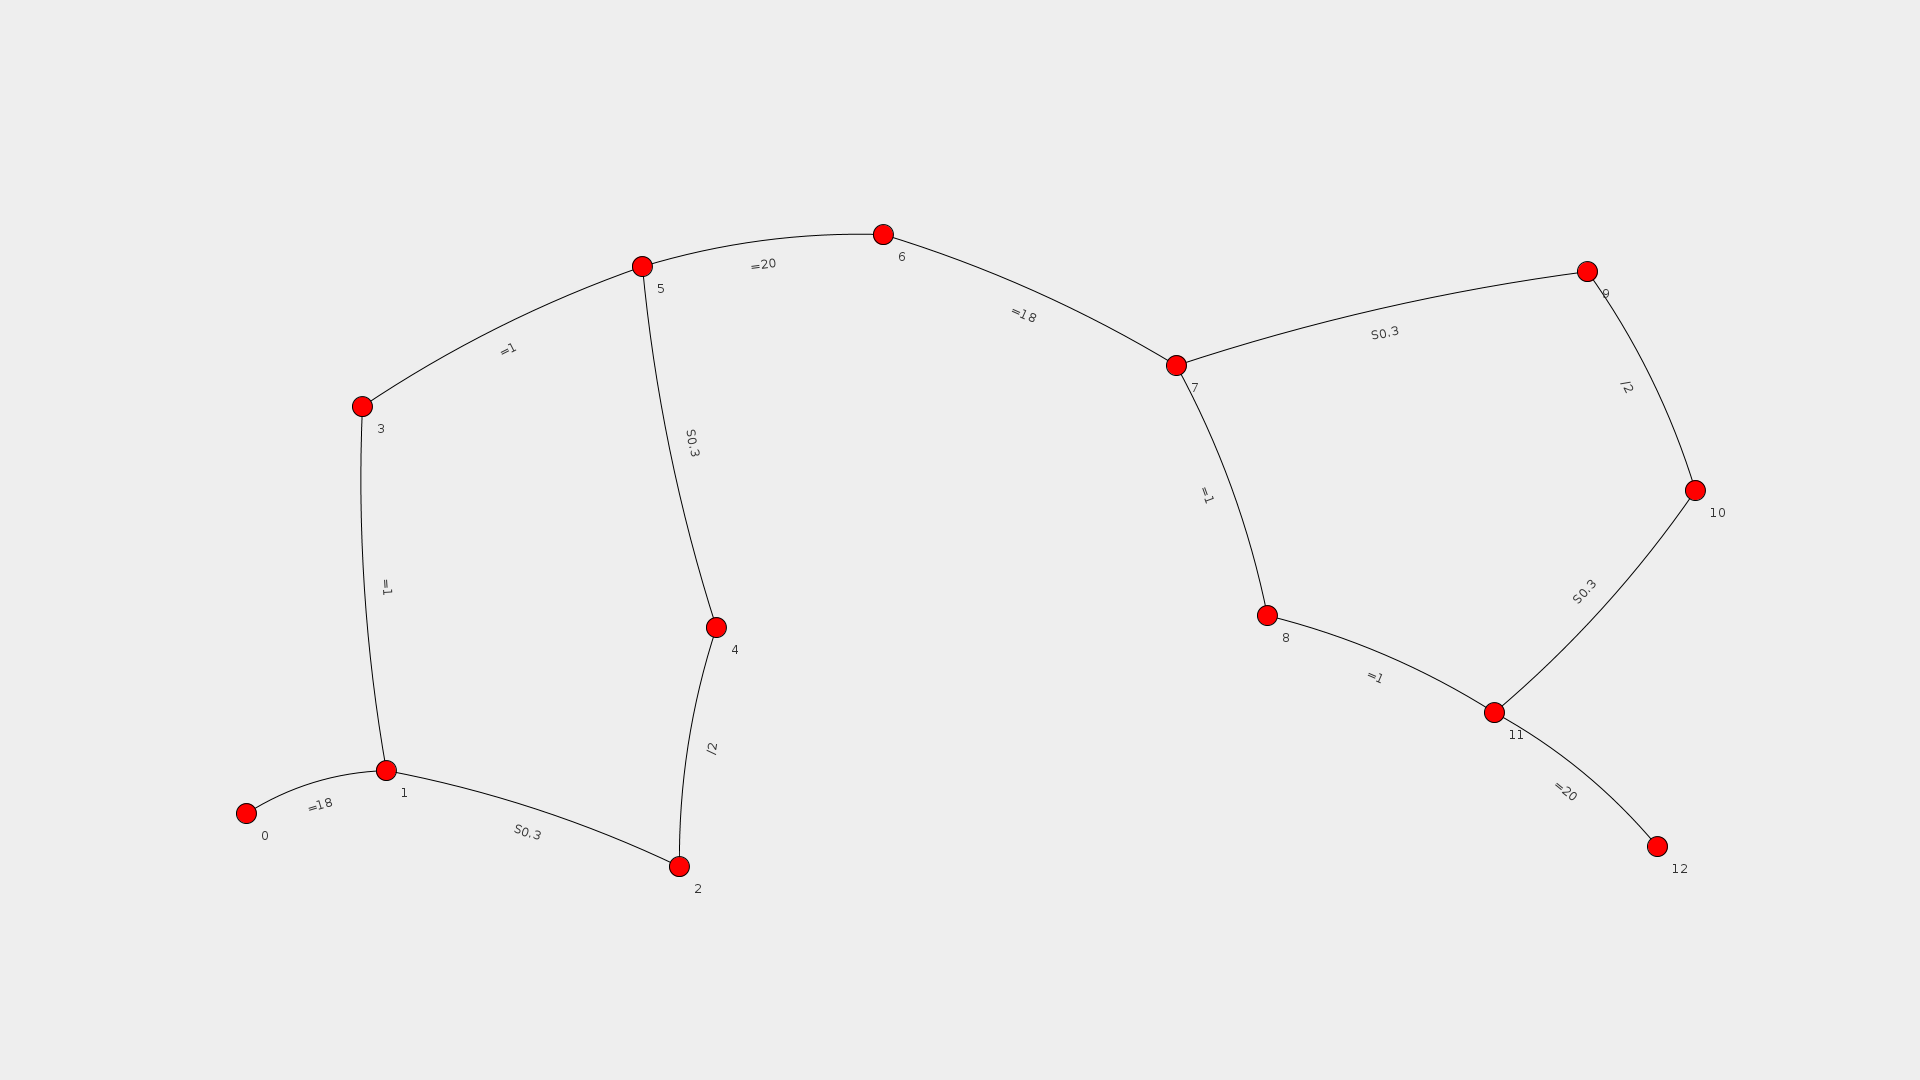
\includegraphics[width=150mm,angle=90]{solution.png}
\caption{RAS DATA SET TOY example territory. Undirected graph, arcs have descriptions.}
\end{figure}

\begin{figure}
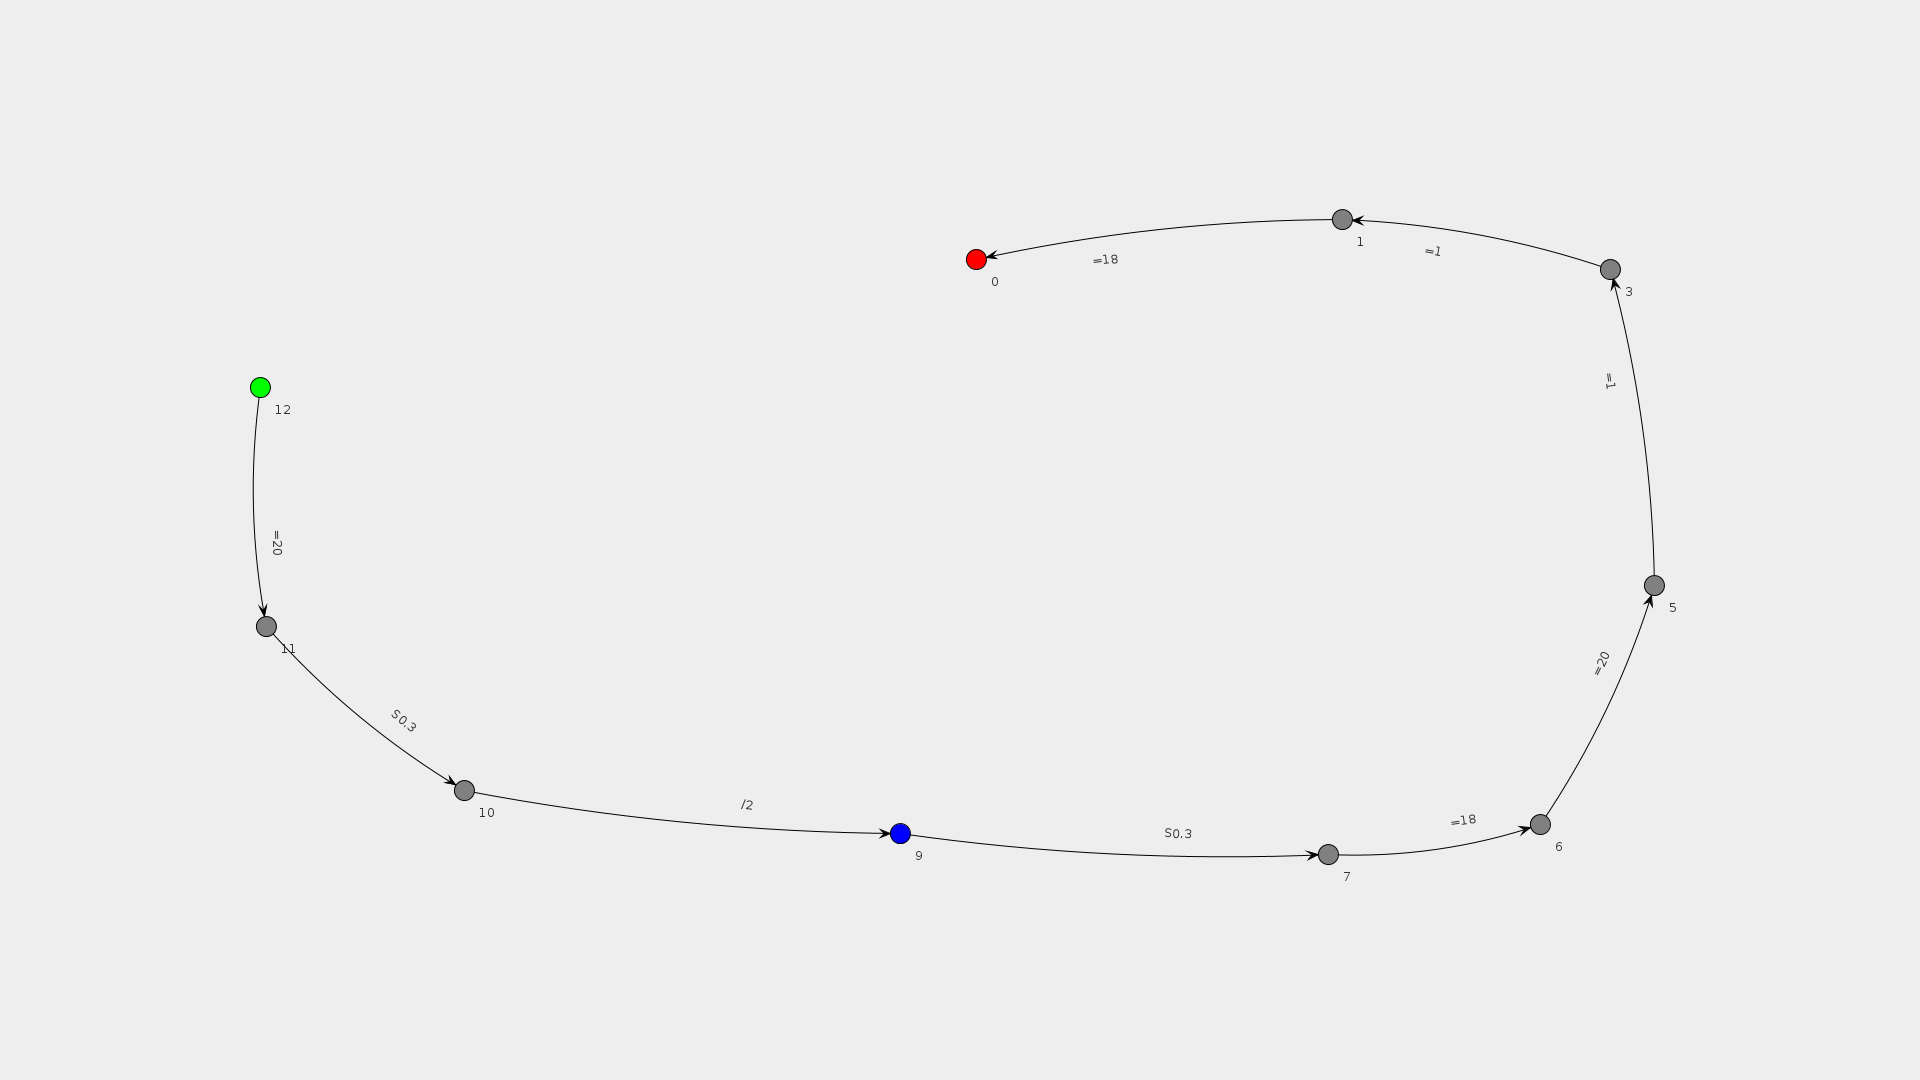
\includegraphics[width=150mm,angle=90]{B1.png}
\centering
\caption{RAS DATA SET TOY example, route of Train B1. Directed graph where green marks the origin, red the destination and blue is where the train is allowed to wait.}
\end{figure}

In this section, we show examples of visualizations that the solution is capable of providing. These visualizations have been rendered on the fly using the JUNG library\footnote{Java Universal Network/Graph framework, http://jung.sourceforge.net}.

\end{document}
